% Copyright © 2015 Martin Ueding <dev@martin-ueding.de>
%
\documentclass[english, fleqn]{beamer}

%\usetheme{default}
\useoutertheme{infolines}

\usecolortheme{whale}
%\usecolortheme{rose}

\usepackage[beamer]{header}

\renewcommand\iup{\text i}
\renewcommand\eup{\text e}

\title{Analysis of $\piup$--$\piup$ scattering data}
%\subtitle{}
\author{Martin Ueding – mu@martin-ueding.de}
\date{2015-03-20}

\AtBeginSection[]
{
    \begin{frame}
        \sectionpage
        \tableofcontents[sectionstyle=show/shaded, subsectionstyle=show/shaded/hide]
    \end{frame}
}

\AtBeginSubsection[]
{
    \begin{frame}
        \subsectionpage
        \tableofcontents[sectionstyle=show/shaded, subsectionstyle=show/shaded/hide]
    \end{frame}
}

\setbeamertemplate{navigation symbols}{}

\begin{document}

\begin{frame}
    \titlepage
\end{frame}

\begin{frame}
    \frametitle{Contents of this presentation}
    \tableofcontents
\end{frame}

%%%%%%%%%%%%%%%%%%%%%%%%%%%%%%%%%%%%%%%%%%%%%%%%%%%%%%%%%%%%%%%%%%%%%%%%%%%%%%%
%                               Data generation                               %
%%%%%%%%%%%%%%%%%%%%%%%%%%%%%%%%%%%%%%%%%%%%%%%%%%%%%%%%%%%%%%%%%%%%%%%%%%%%%%%

\section{Data generation}

\subsection{Metropolis algorithm}

\subsection{Correlation functions}

%%%%%%%%%%%%%%%%%%%%%%%%%%%%%%%%%%%%%%%%%%%%%%%%%%%%%%%%%%%%%%%%%%%%%%%%%%%%%%%
%                              Analysis methods                               %
%%%%%%%%%%%%%%%%%%%%%%%%%%%%%%%%%%%%%%%%%%%%%%%%%%%%%%%%%%%%%%%%%%%%%%%%%%%%%%%

\section{Analysis methods}

\newcommand\scale{0.2}

\subsection{Importing data}

\begin{frame}
    \frametitle{Input data}
    \begin{center}
        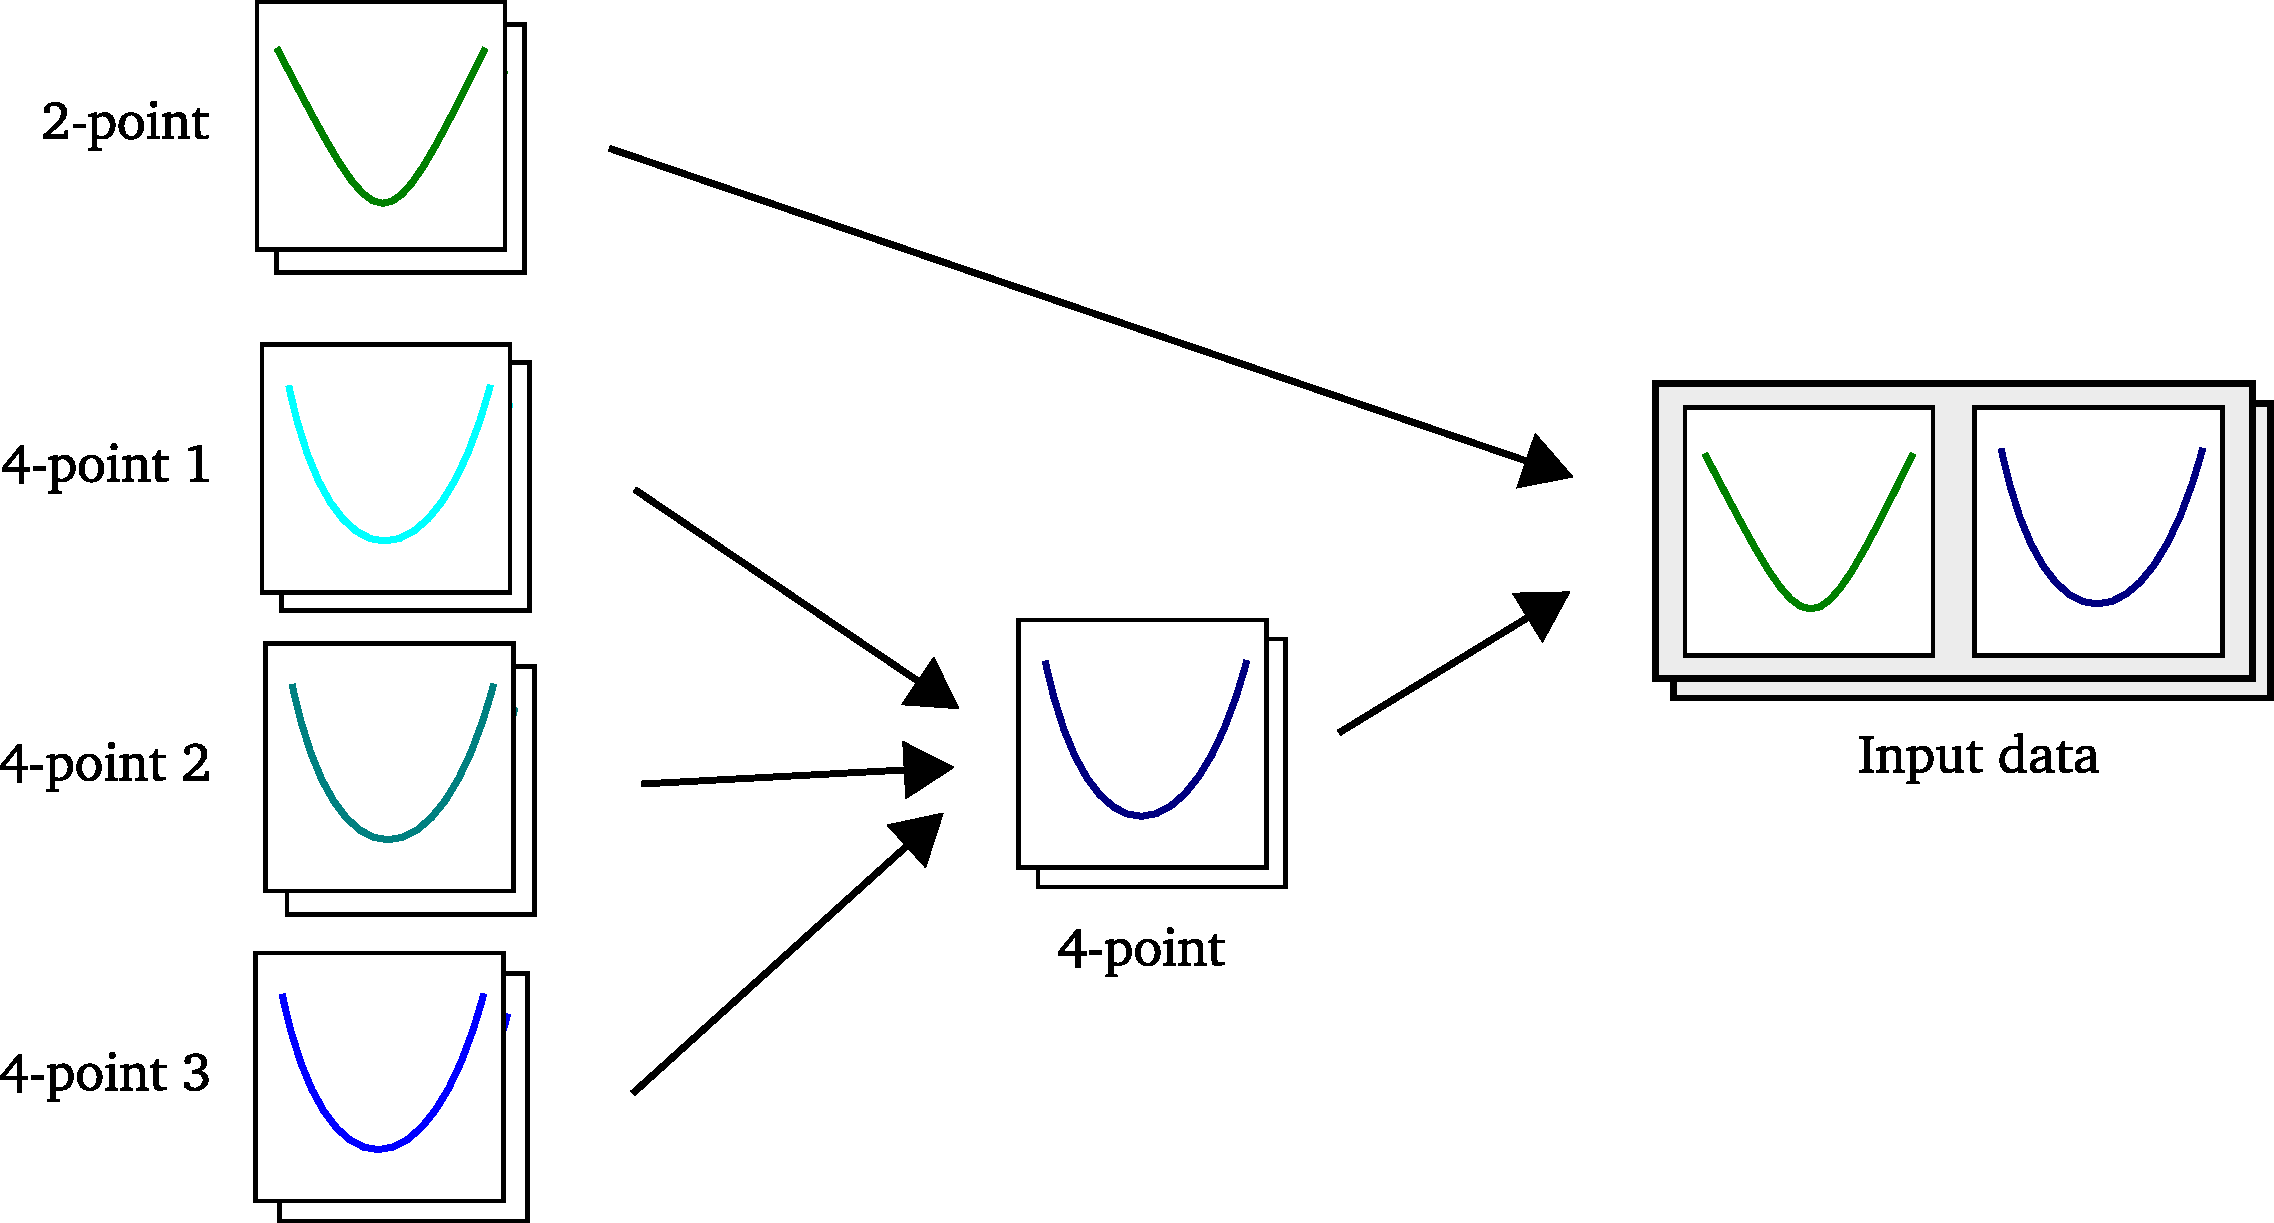
\includegraphics[scale=\scale]{sketches/01-input.pdf}
    \end{center}
\end{frame}

\begin{frame}
    \frametitle{Folding}
    \begin{center}
        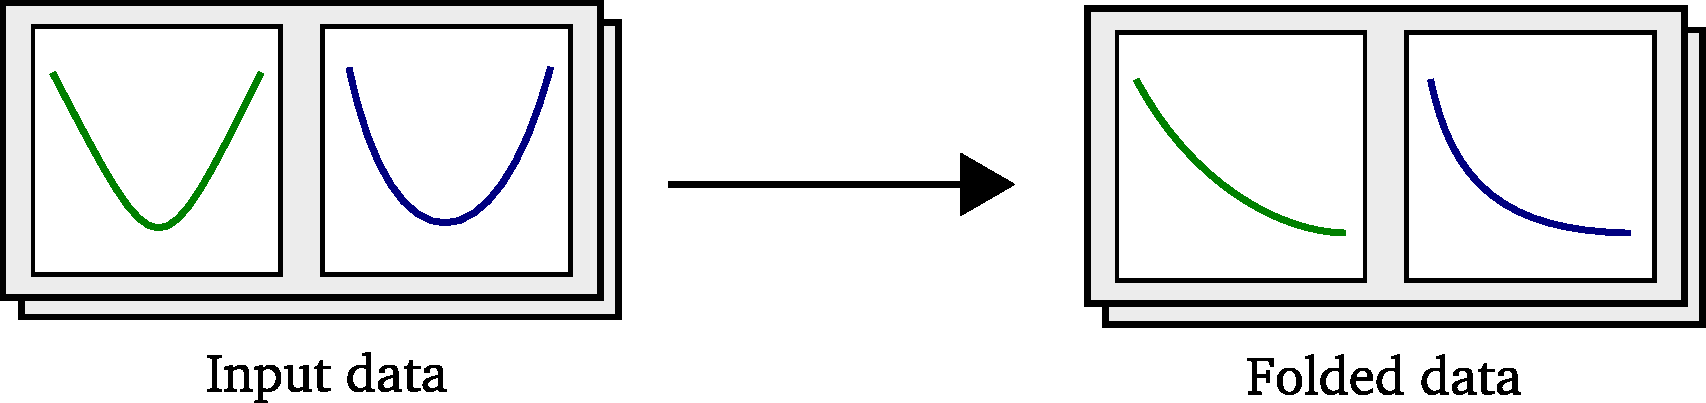
\includegraphics[scale=\scale]{sketches/02-folding.pdf}
    \end{center}
\end{frame}

\subsection{Bootstrap}

\begin{frame}
    \frametitle{Alternatives?}
    Gaussian error propagation …
    \begin{itemize}
        \item
            is tedious
        \item
            assumes small errors
        \item
            does not scale
    \end{itemize}
\end{frame}

\begin{frame}
    \frametitle{A quick review}
    The bootstrap method:
    \begin{itemize}
        \item
            Analysis function $f$: Transforms input data $X$ into output data
            $Y$ \\
            E.g. samples $X = \{x_i\}$ to median $Y$
        \item
            $f(X)$ is estimate for value
        \item
            Generate $R$ samples from $X$: $\{\tilde X_i\}_i$
        \item
            Apply $f$ to each sample: $\{f(\tilde X_i)\}_i$
        \item
            Error is standard deviation: $\Deltaup Y = \sigma(\{f(\tilde X_i)\}_i)$
    \end{itemize}

    Value and error without computing derivatives!
\end{frame}

\begin{frame}
    \frametitle{Generation of bootstrap samples}
    \begin{center}
        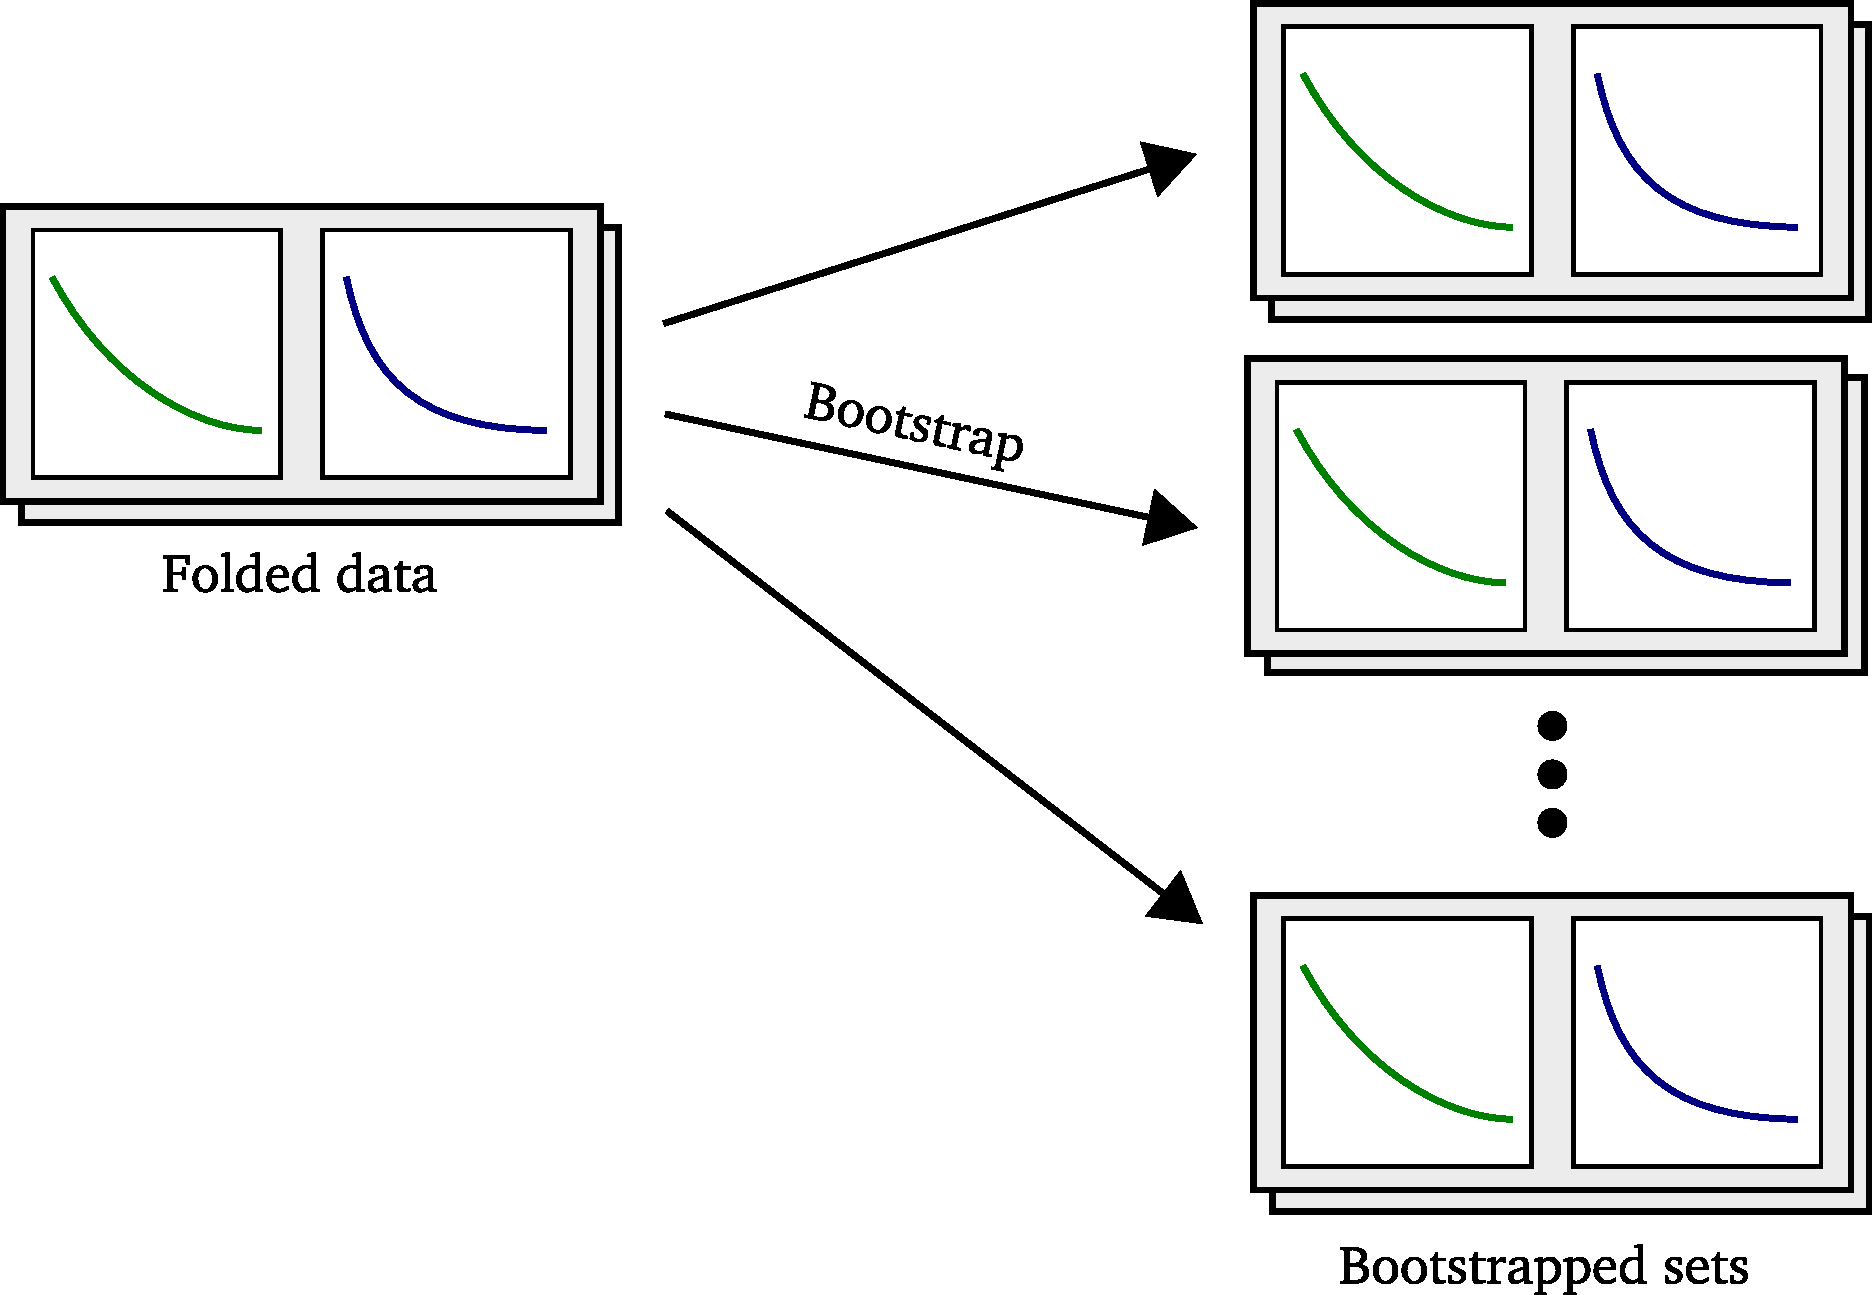
\includegraphics[scale=\scale]{sketches/03-bootstrap.pdf}
    \end{center}
\end{frame}

\begin{frame}
    \frametitle{Averaging for further analysis}
    \begin{center}
        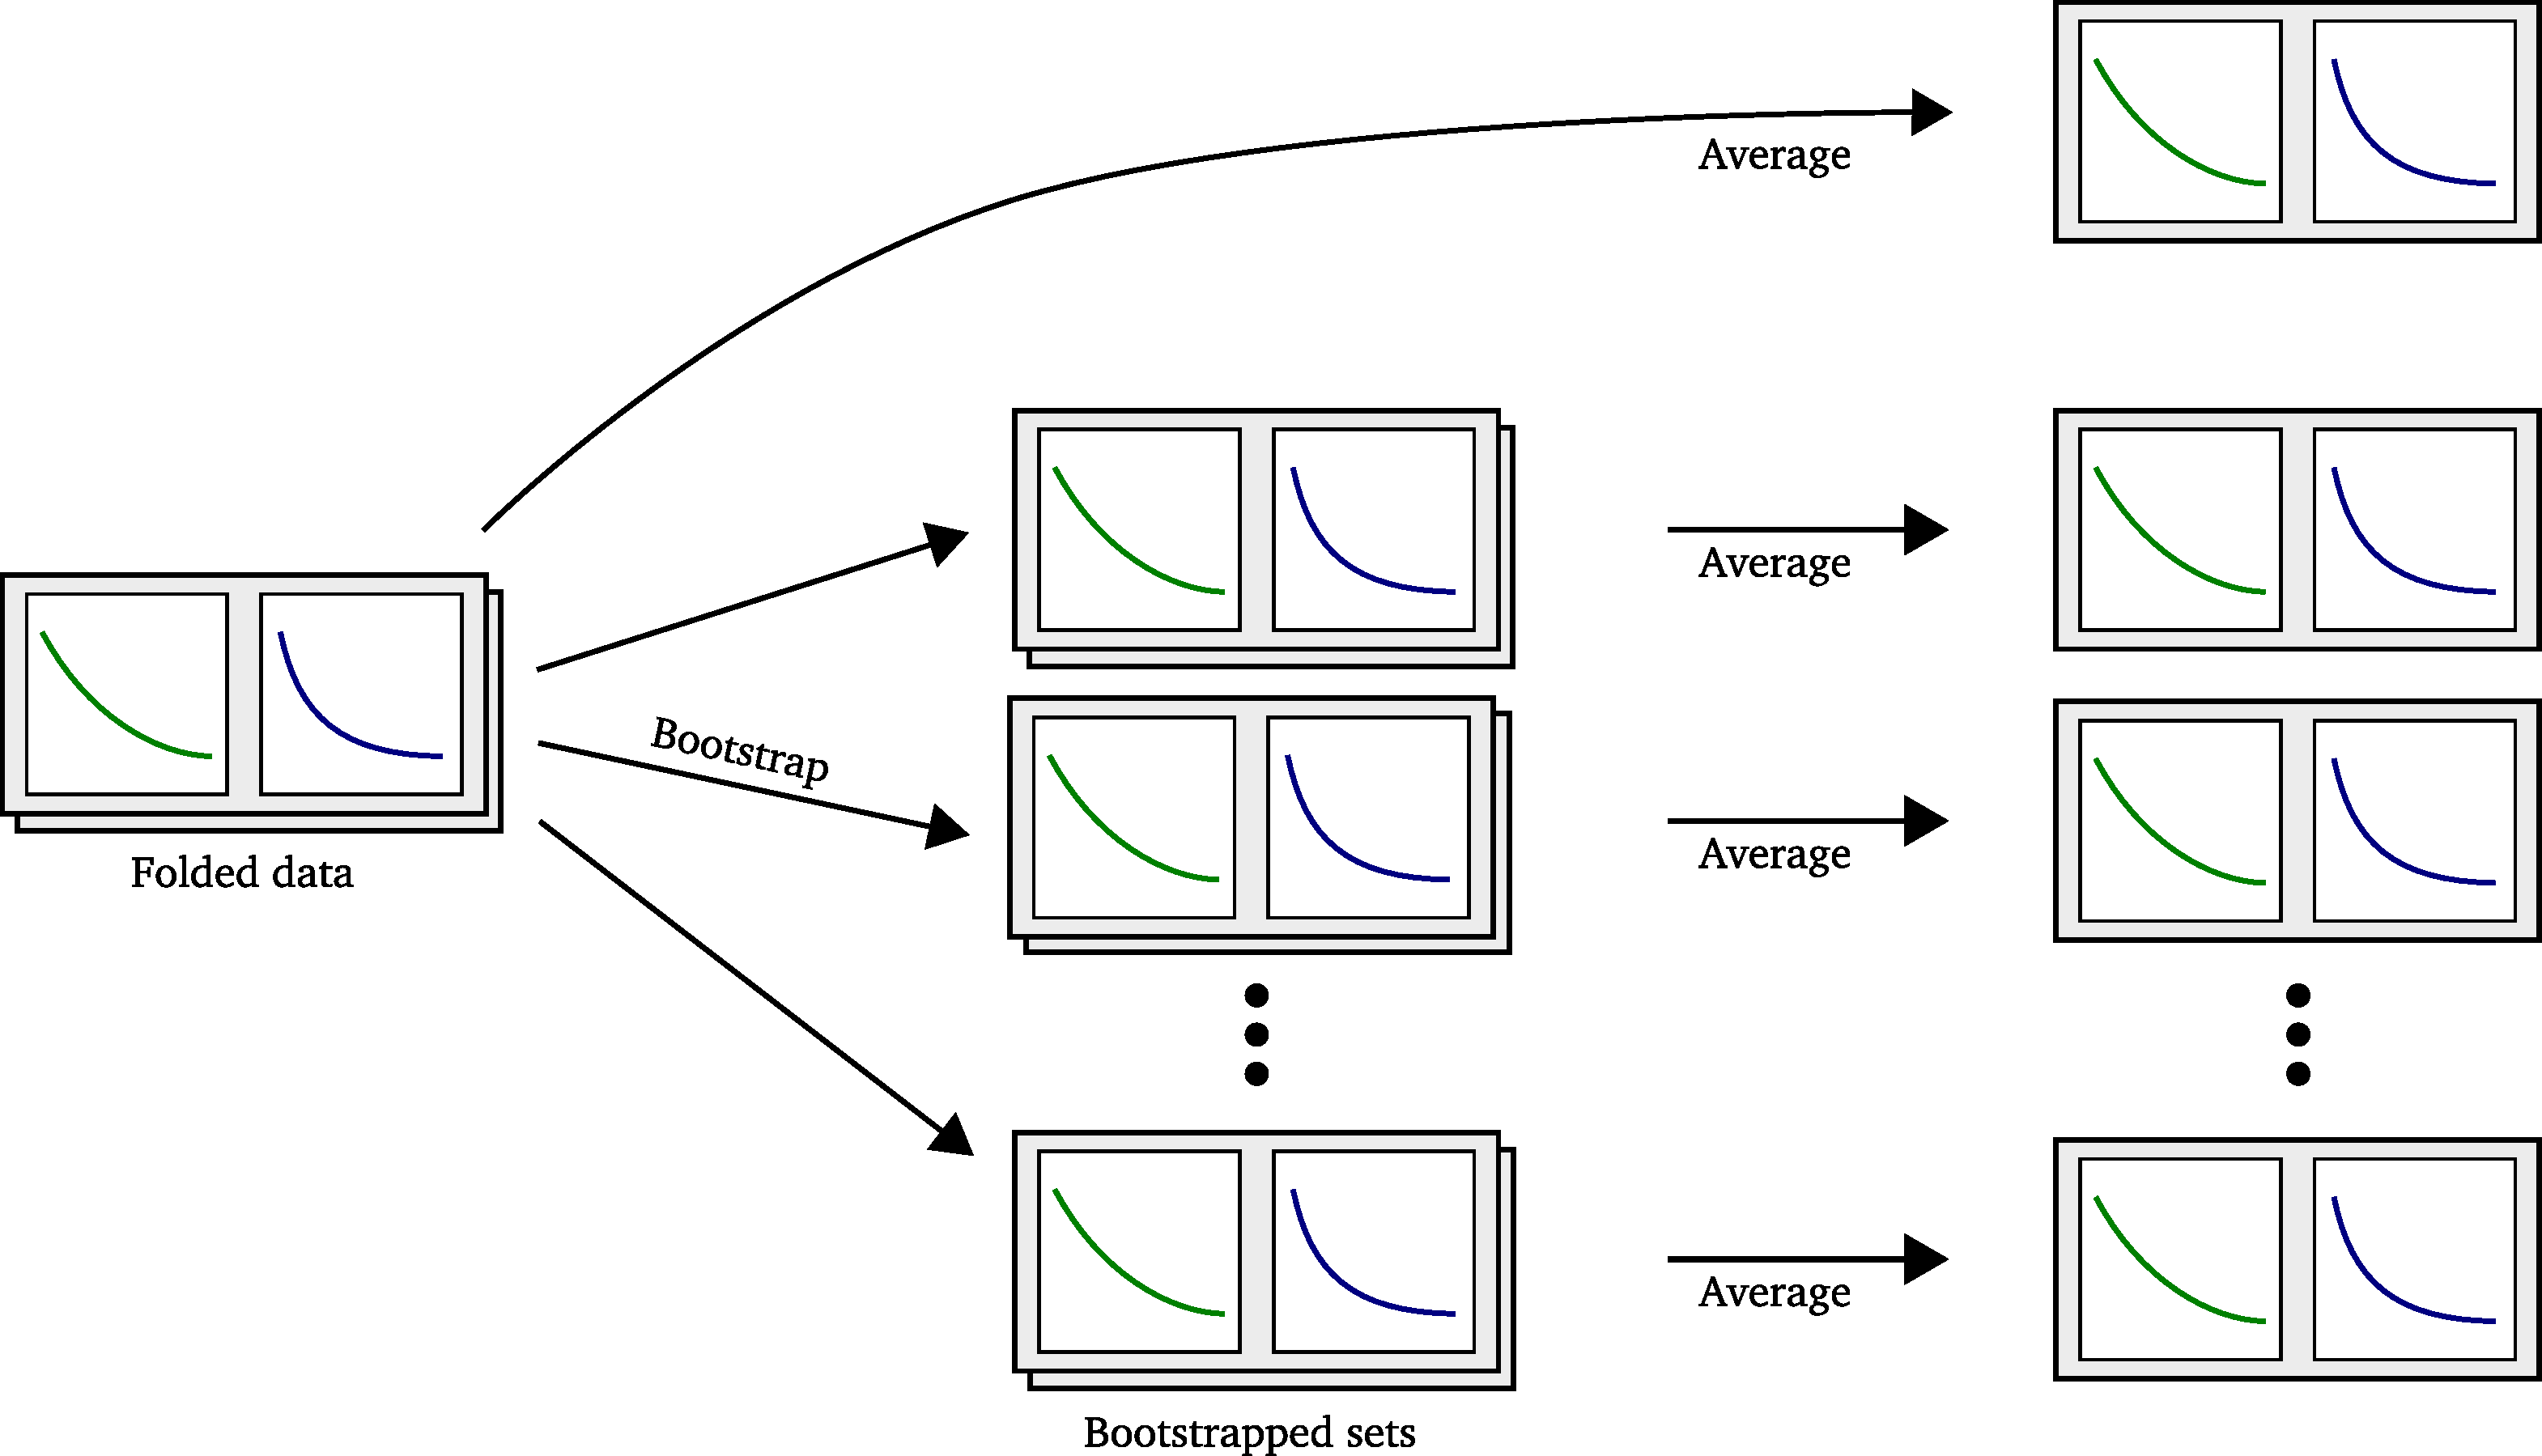
\includegraphics[scale=\scale]{sketches/04-bootstrap.pdf}
    \end{center}
\end{frame}

\subsection{Correlated fit}

\begin{frame}
    \frametitle{Correlation in data points}
    \begin{itemize}
        \item
            Markov chain data is correlated
        \item
            Regular fit will give wrong $\chi^2$ and $p \approx 1$
        \item
            Correlated fit is needed
    \end{itemize}
\end{frame}

\begin{frame}
    \frametitle{New $\chi^2$}

    New $\chi^2$:
    \[
        \chi^2 := \sum_{i, j}^T
        \left[ \bar x_{iN} - f(t_i, \lambda) \right]
        C^{-1}_{ij}
        \left[ \bar x_{jN} - f(t_j, \lambda) \right]
        \eqnsep
        \bar x_{iN} := \frac 1N \sum_{n=1}^N x_{in}
    \]
    Correlation matrix:
    \[
        C_{ij} := \frac{1}{N[N-1]} \sum_{k=1}^N
        [x_{ik} - \bar x_{iN}] [x_{jk} - \bar x_{jN}]
    \]

    \begin{description}
        \item[$\lambda$] Fit parameters
        \item[$i$, $j$] Time slice number
        \item[$N$] Number of measurements
    \end{description}
\end{frame}

\begin{frame}
    \frametitle{Correlation matrix with less indices}

    \begin{align*}
        C_{ij}
        &= \frac{1}{N[N-1]} \sum_{k=1}^N [x_{ik} - \bar x_{iN}] [x_{jk} - \bar x_{jN}] \\
        &= \frac{1}{N[N-1]} \sum_{k=1}^N d_{ik} d_{jk} & d_{ik} := x_{ik} - \bar x_{iN} \\
        &= \frac{1}{N[N-1]} \sum_{k=1}^N d_{ik} d_{kj}^{\text T} \\
        &= \frac{1}{N[N-1]} \vec d_{i} \vec d_{j}^{\text T} \\
    \end{align*}
\end{frame}

\begin{frame}
    \frametitle{Correlation matrix}
    \begin{center}
        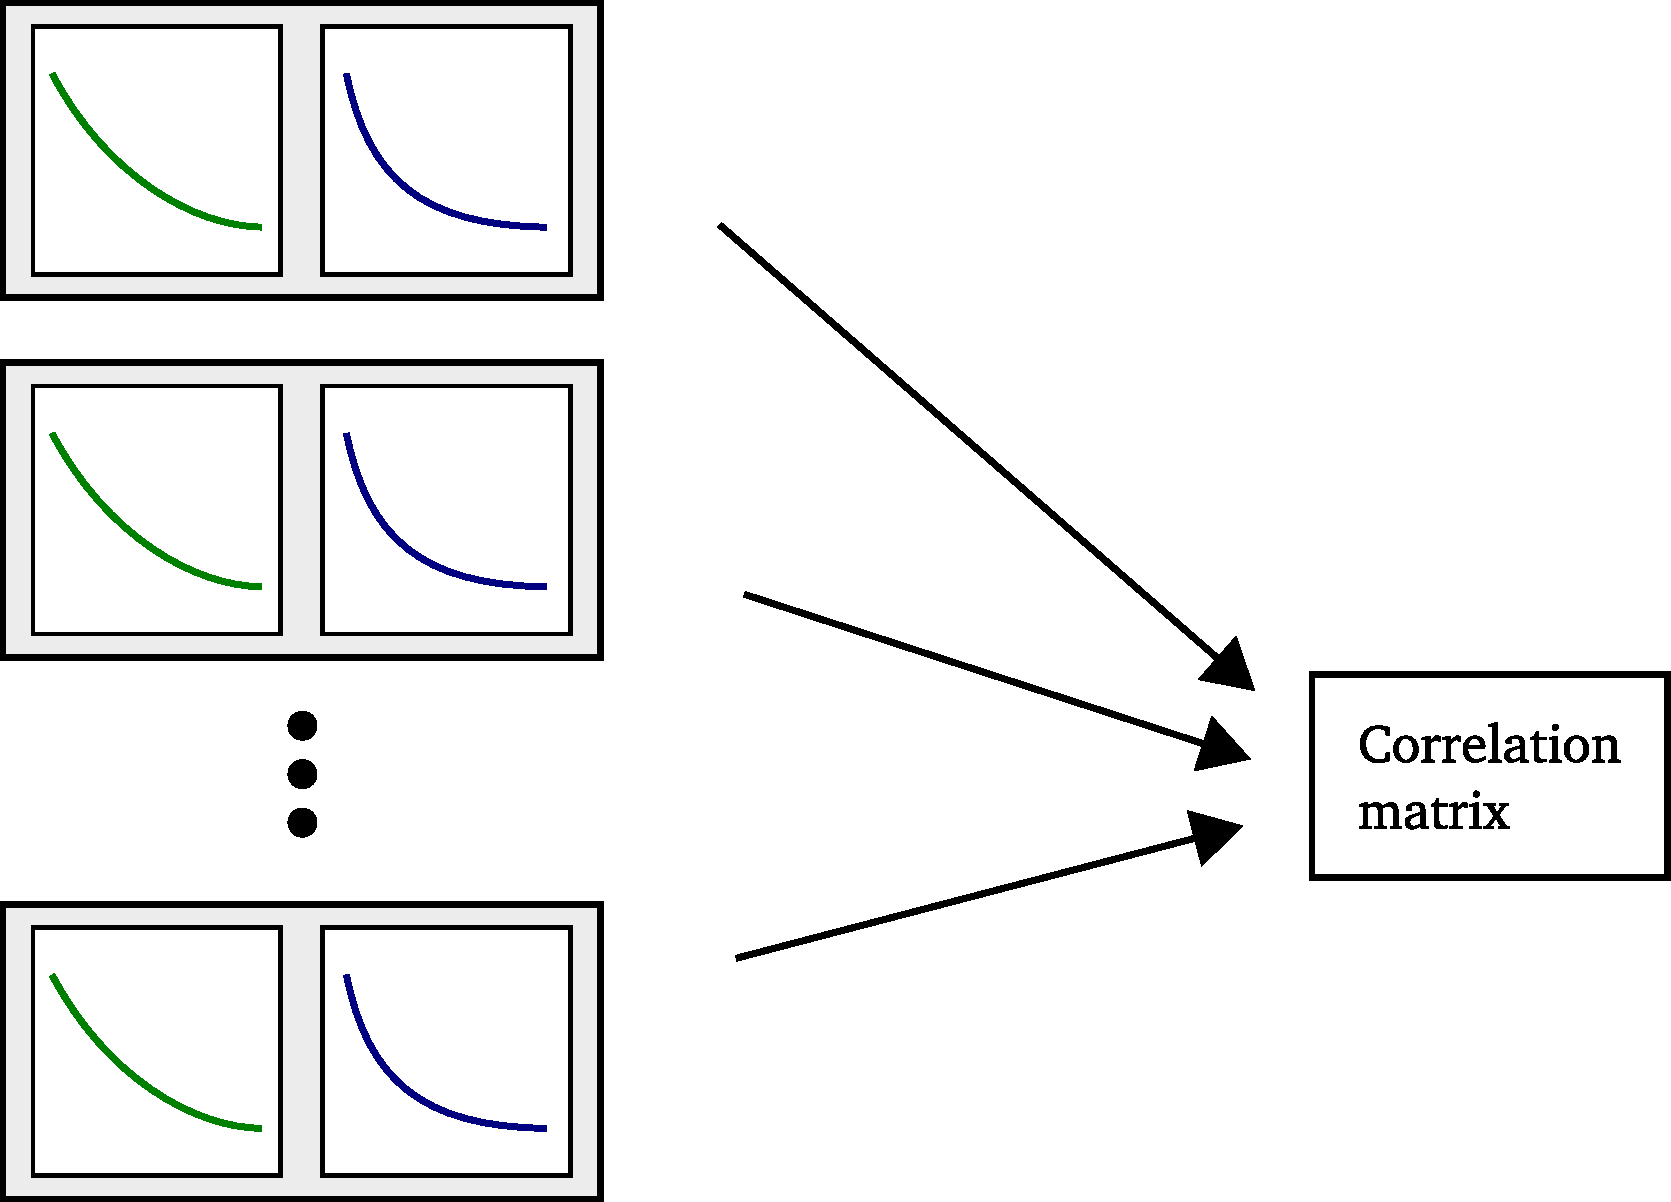
\includegraphics[scale=\scale]{sketches/05-matrix.pdf}
    \end{center}
\end{frame}

\begin{frame}
    \frametitle{$\chi^2$ with less indices}

    \begin{align*}
        \chi^2
        &= \sum_{i, j}^T
        \left[ \bar x_{iN} - f(t_i, \lambda) \right]
        C^{-1}_{ij}
        \left[ \bar x_{jN} - f(t_j, \lambda) \right] \\
        &= 
        \vec r^{\text T}
        \vec C^{-1}
        \vec r
        &
        r_i := \bar x_{iN} - f(t_i, \lambda)
        \\
    \end{align*}

    Comparison: Plain $\chi^2$ is
    \[
        \chi^2 = |\vec r|^2 = \vec r^{\text T} \vec r
    \]
\end{frame}

\begin{frame}
    \frametitle{Correlated fit}
    \begin{center}
        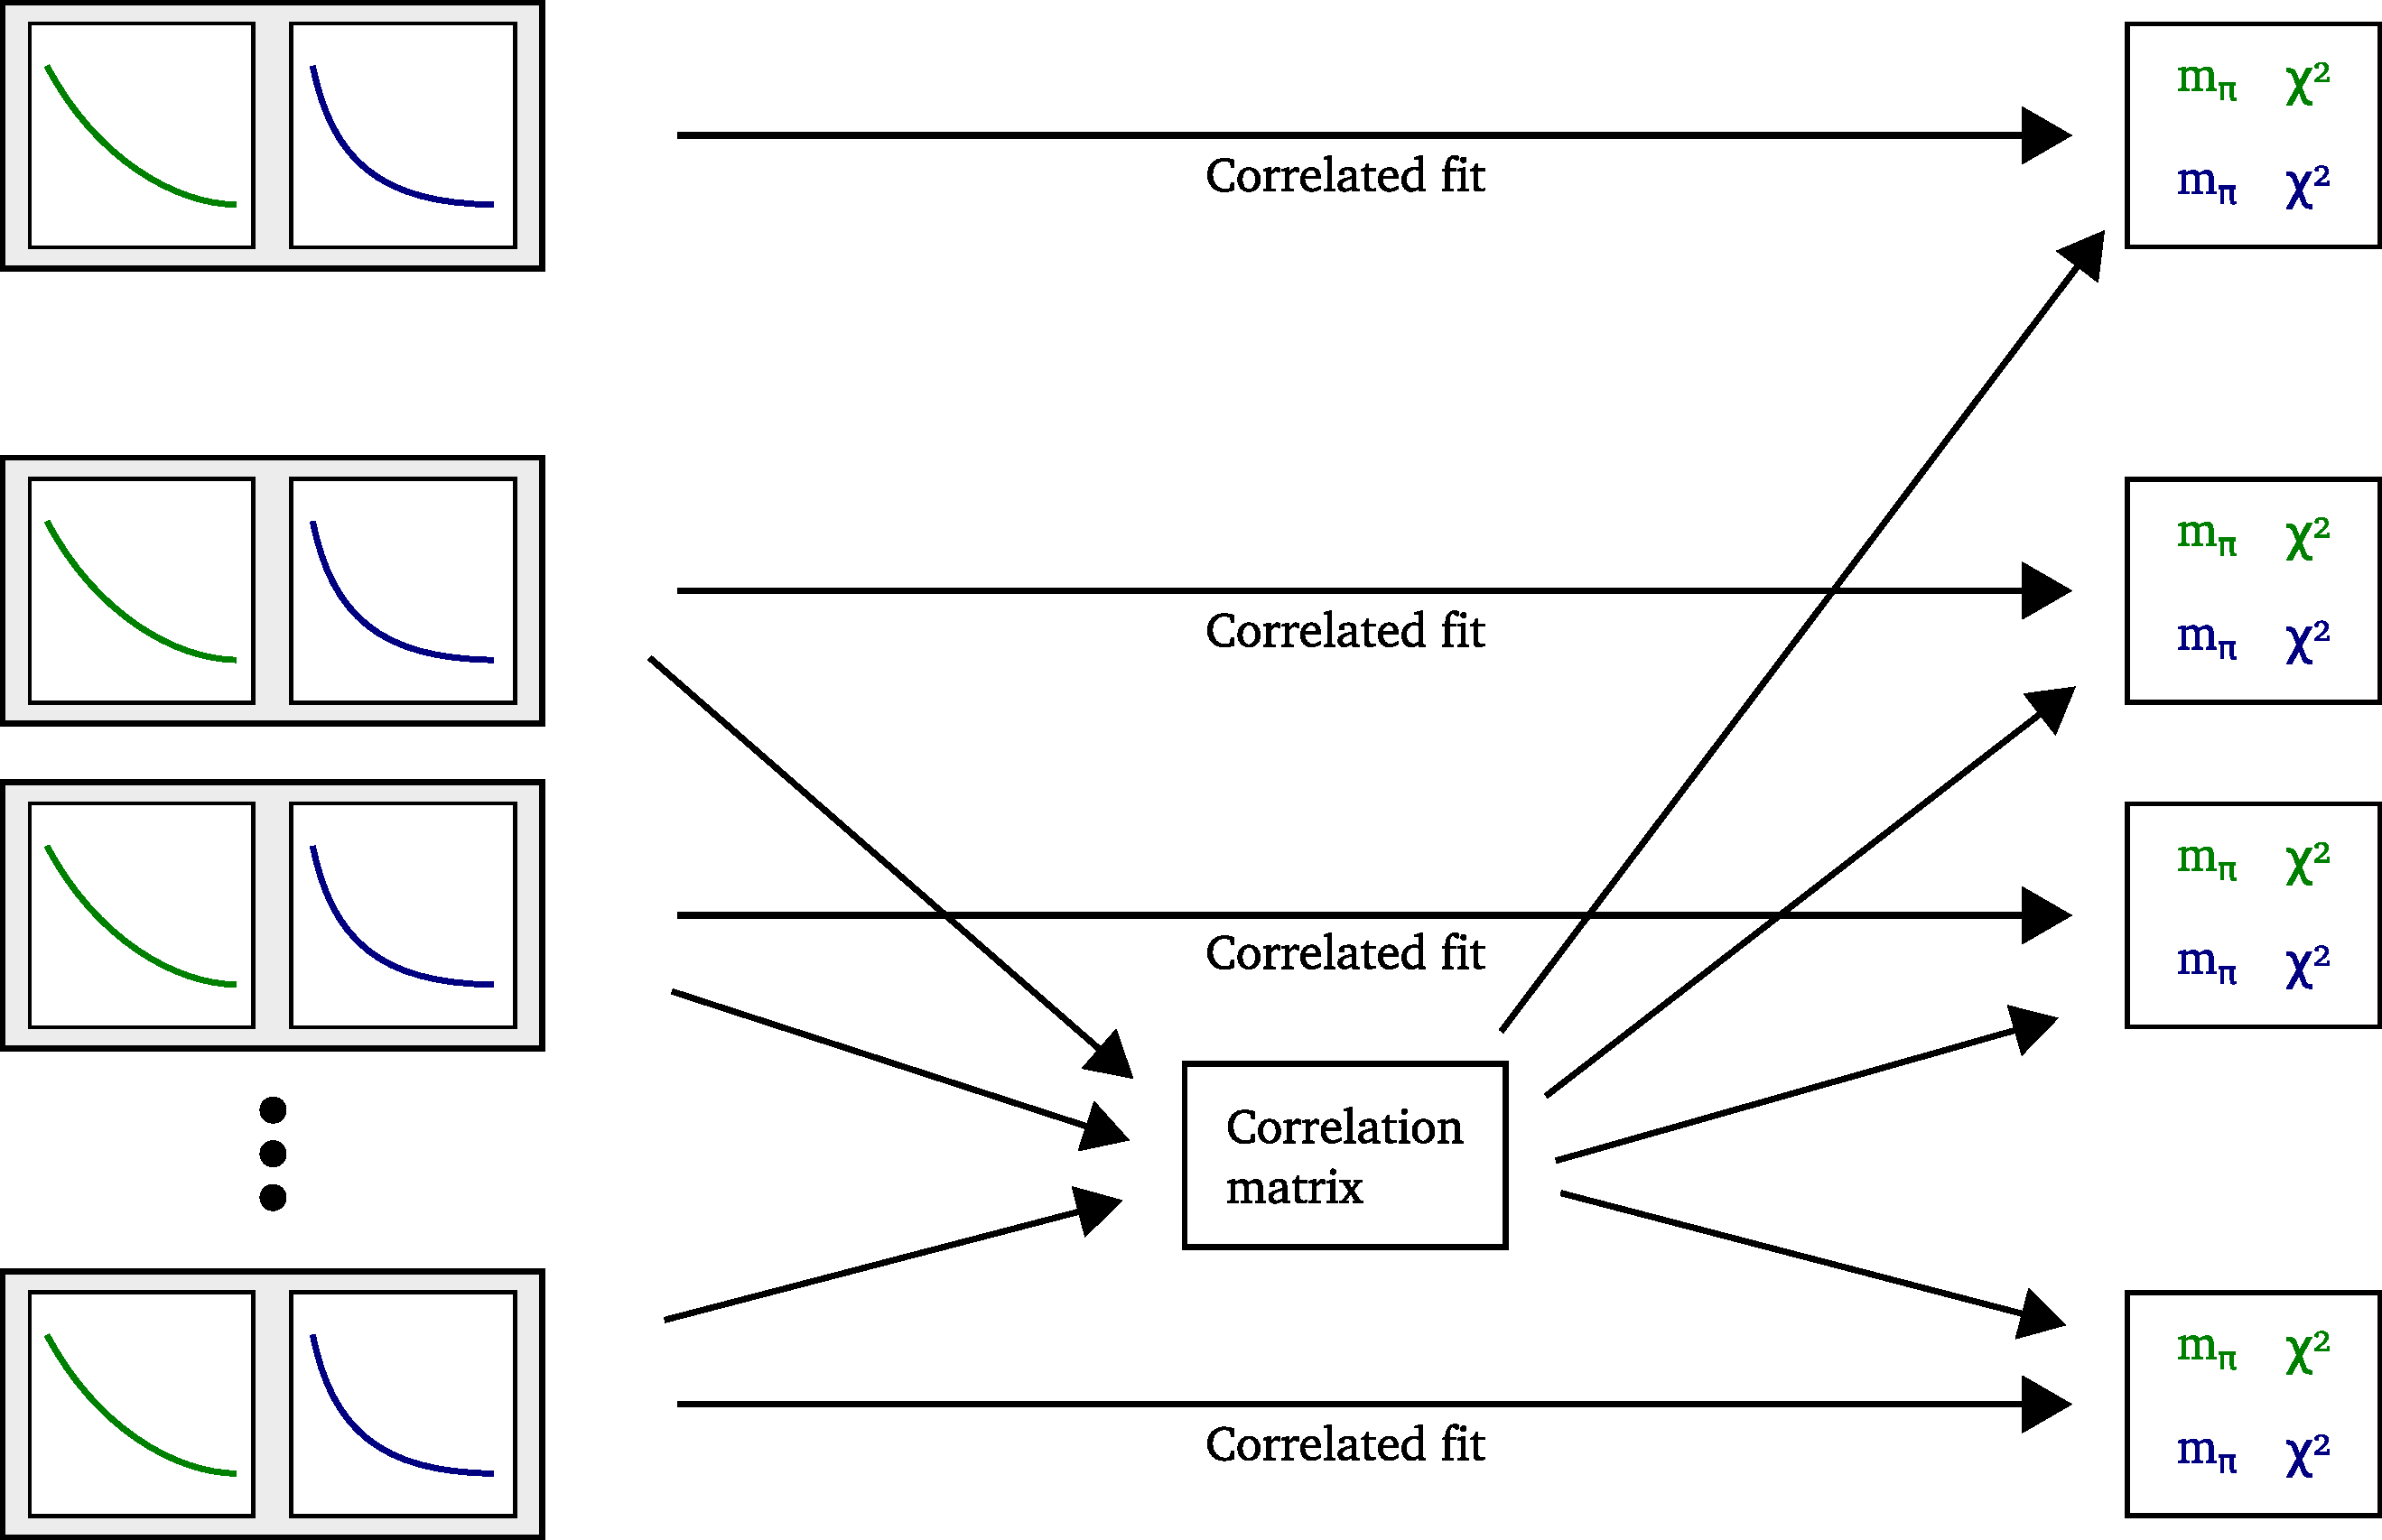
\includegraphics[scale=\scale]{sketches/06-fit.pdf}
    \end{center}
\end{frame}

\subsection{Scattering length}

\begin{frame}
    \frametitle{From masses to scattering length}

    There is a relation between mass difference to scattering length
    \parencite[(1.3)]{luescher/volume_dependence}:
    \[
        W = 2m - \frac{4 \piup a_0}{m L^3} \sbr{1 + c_1 \frac{a_0}L + c_2 \frac{a_0^2}{L^2}}
    \]

    \begin{description}
        \item[$W$] Mass of $\piup$-$\piup$-system
        \item[$m$] Mass of single $\piup$
        \item[$a_0$] s-wave scattering length
        \item[$L$] Number of spatial lattice sites
        \item[$c_1$] \num{-2.837297}
        \item[$c_2$] \num{6.375183}
    \end{description}
\end{frame}

\begin{frame}
    \frametitle{Derivation of Lüscher's formula}

    % TODO
\end{frame}

\begin{frame}
    \frametitle{Application of Lüscher's formula}
    \begin{columns}
        \begin{column}{0.6\textwidth}
                
            Solve for $a_0$
            \[
                2m - W - \frac{4 \piup a_0}{m L^3} \sbr{1 + c_1 \frac{a_0}L + c_2 \frac{a_0^2}{L^2}} = 0
            \]
            using root finding like
            \begin{itemize}
                \item
                    Newton from $a_0 = 0$
                \item
                    Brent (1973)
            \end{itemize}

        \end{column}
        \begin{column}{0.4\textwidth}
            \begin{center}
                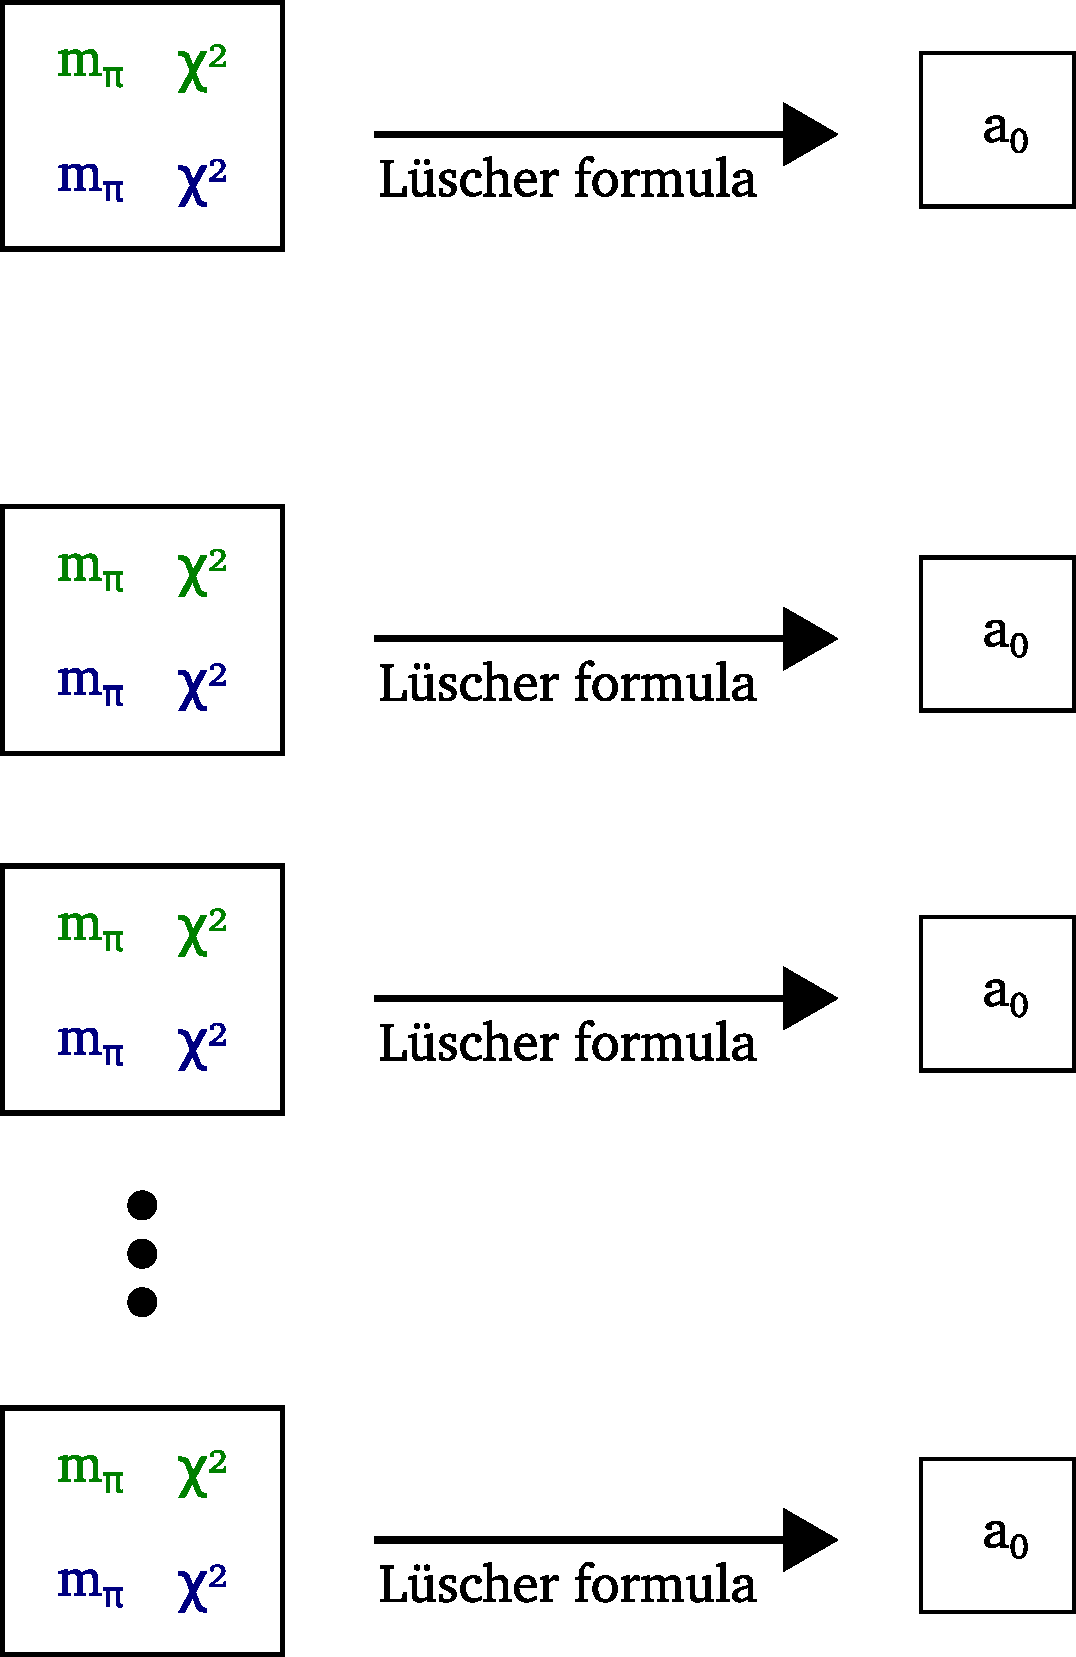
\includegraphics[scale=\scale]{sketches/07-luescher.pdf}
            \end{center}
        \end{column}
    \end{columns}
\end{frame}

\begin{frame}
    \frametitle{End results}
    \begin{center}
        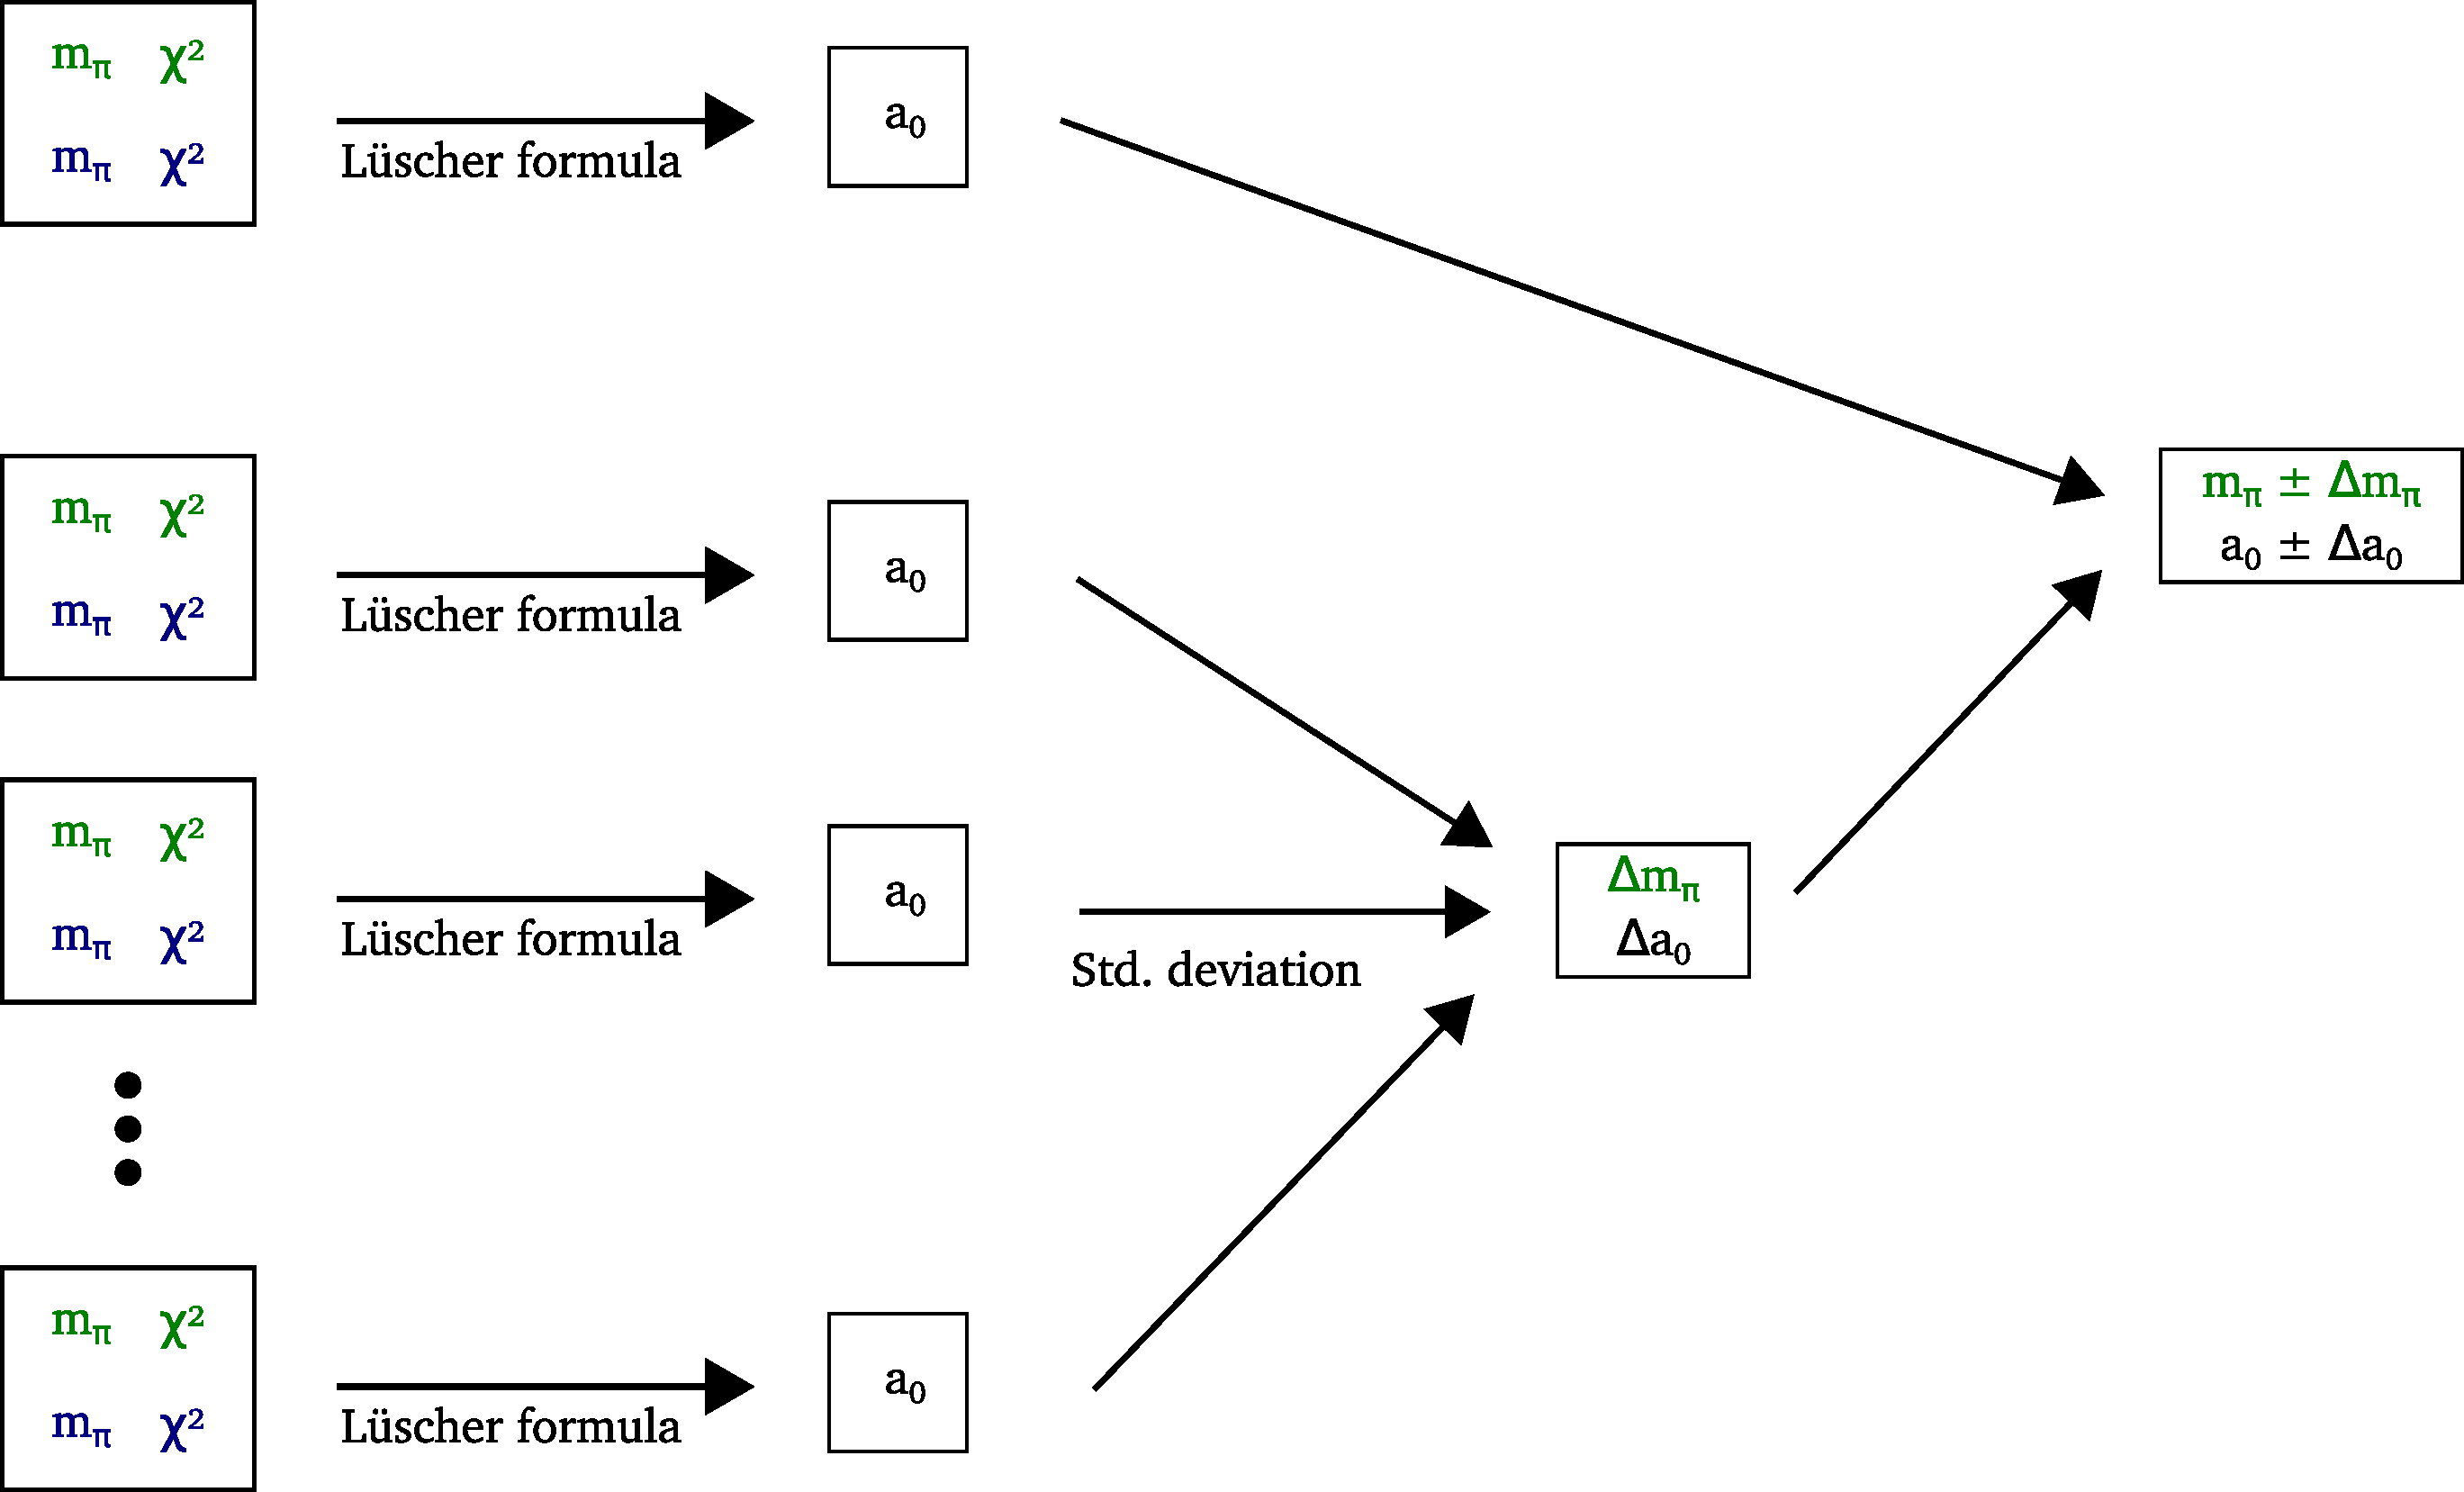
\includegraphics[scale=\scale]{sketches/08-end-result.pdf}
    \end{center}
\end{frame}

%%%%%%%%%%%%%%%%%%%%%%%%%%%%%%%%%%%%%%%%%%%%%%%%%%%%%%%%%%%%%%%%%%%%%%%%%%%%%%%
%                                   Results                                   %
%%%%%%%%%%%%%%%%%%%%%%%%%%%%%%%%%%%%%%%%%%%%%%%%%%%%%%%%%%%%%%%%%%%%%%%%%%%%%%%

\section{Results}

\subsection*{Correlation functions}

\begin{frame}
    \begin{center}
        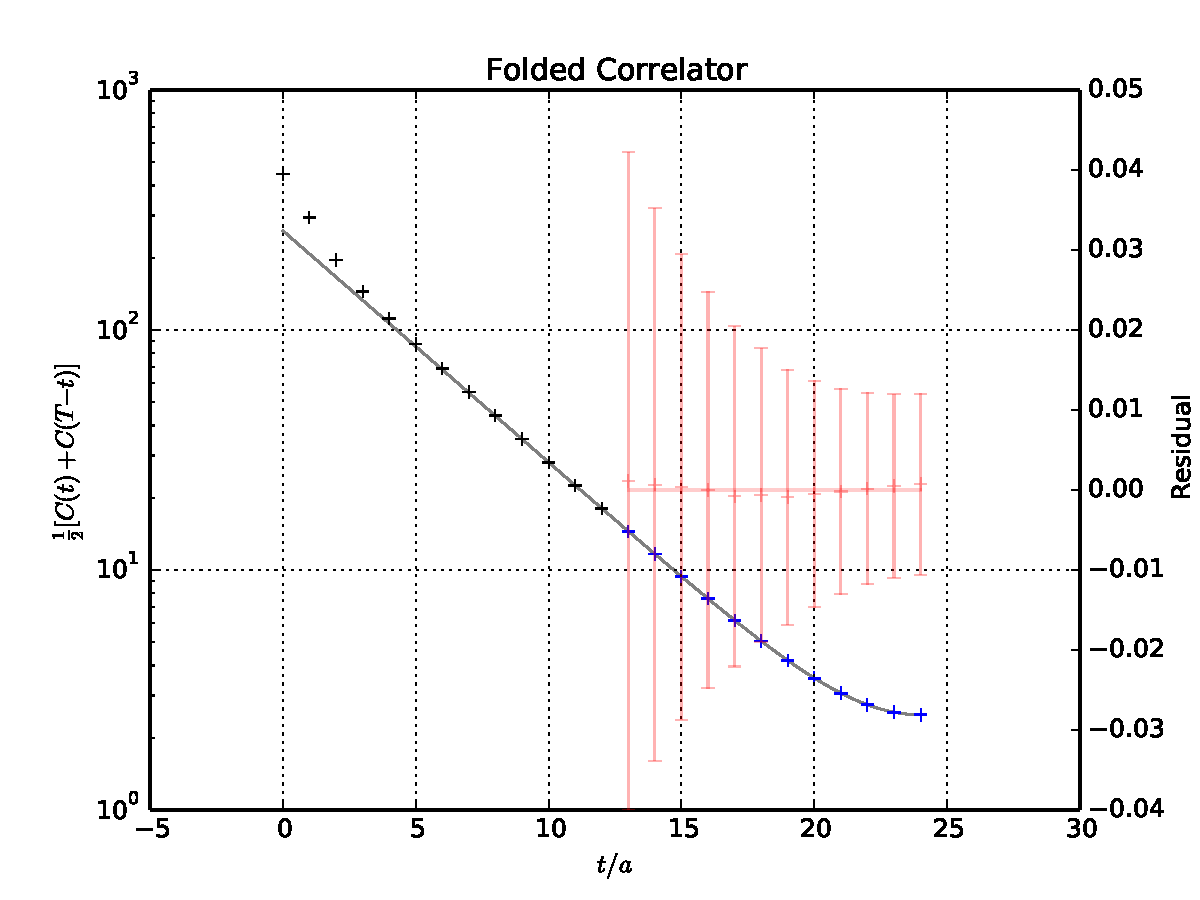
\includegraphics[height=\textheight]{plots/A100_24_L24_T48_beta190_mul0100_musig150_mudel190_kappa1632550__ev120__TB2_SO_LI6_new_c2_folded.pdf}
    \end{center}
\end{frame}

\begin{frame}
    \begin{center}
        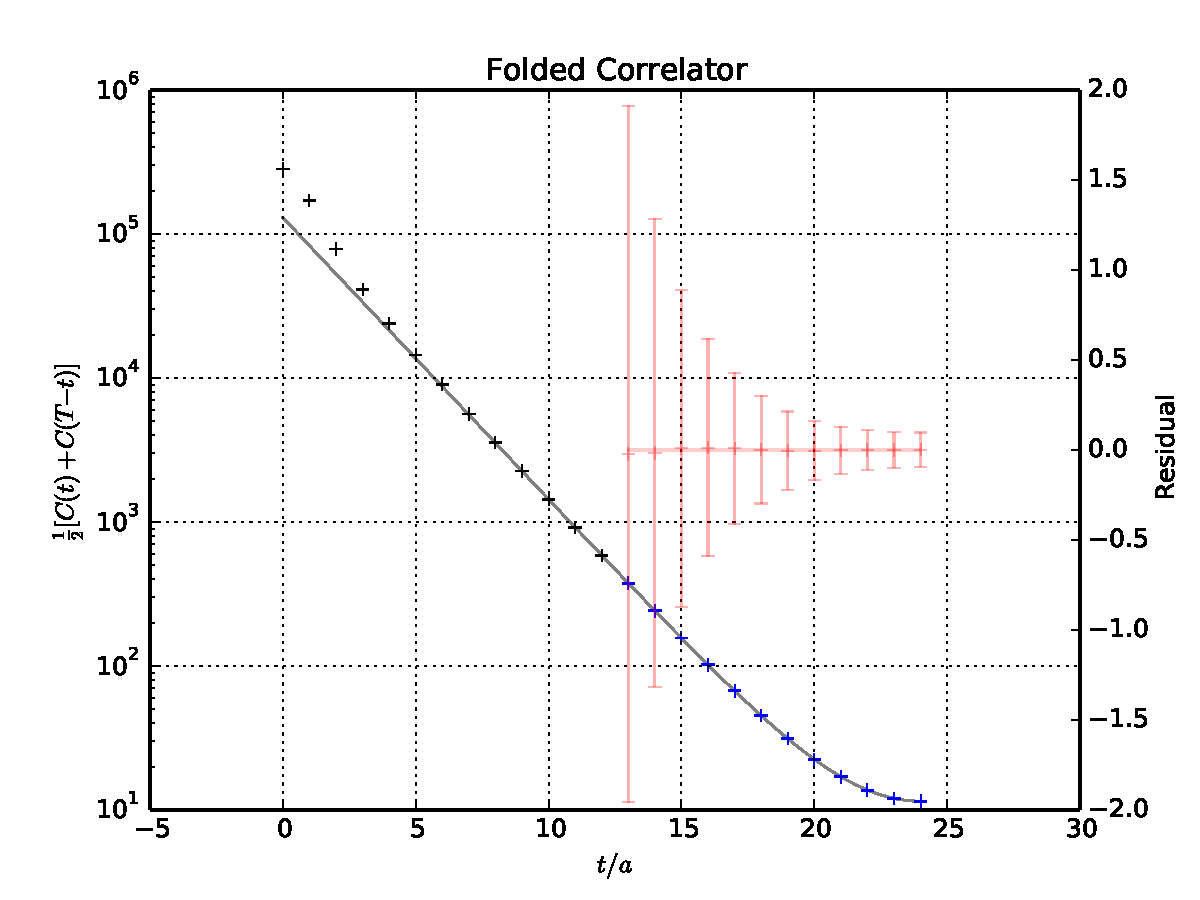
\includegraphics[height=\textheight]{plots/A100_24_L24_T48_beta190_mul0100_musig150_mudel190_kappa1632550__ev120__TB2_SO_LI6_new_c4_folded.pdf}
    \end{center}
\end{frame}

\subsection*{Effective mass}

\begin{frame}
    \begin{center}
        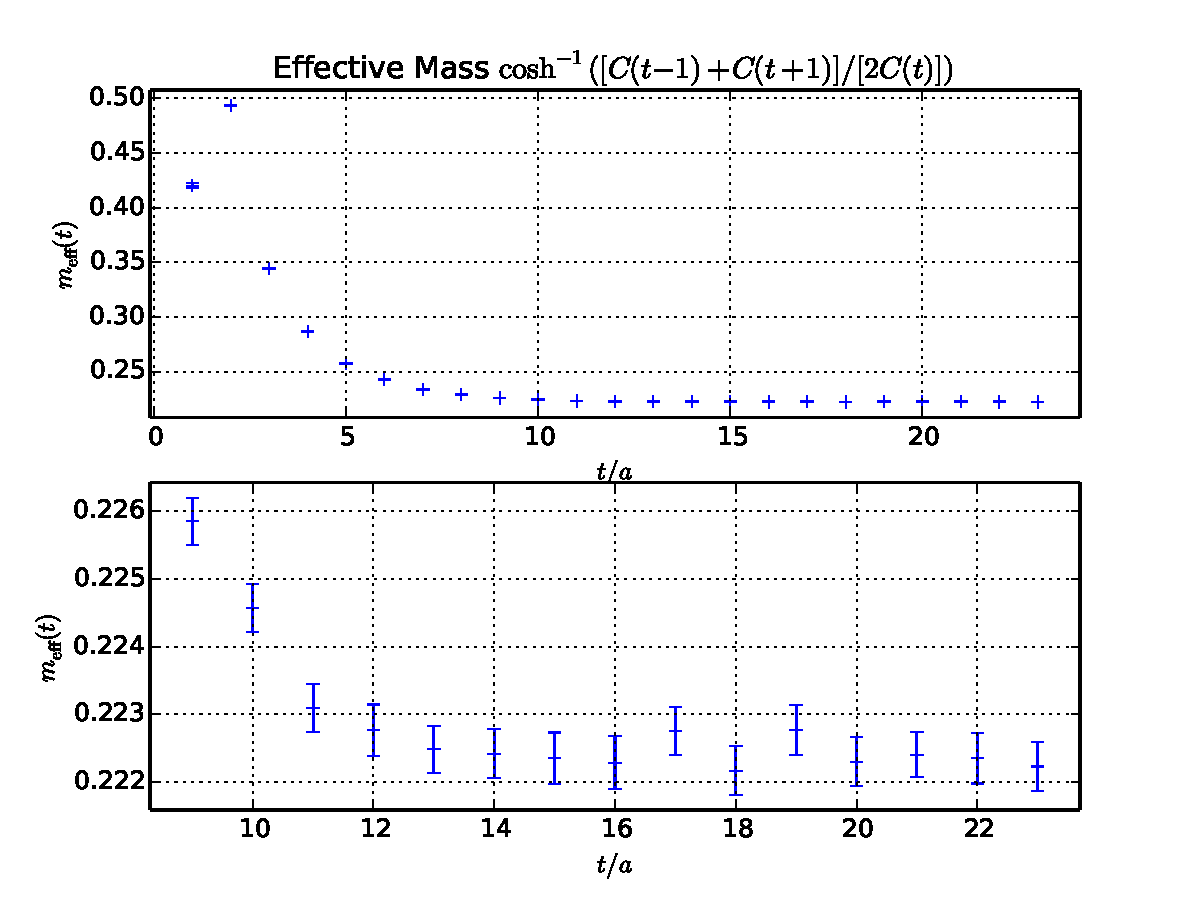
\includegraphics[height=\textheight]{plots/A100_24_L24_T48_beta190_mul0100_musig150_mudel190_kappa1632550__ev120__TB2_SO_LI6_new_c2_m_eff.pdf}
    \end{center}
\end{frame}

\begin{frame}
    \begin{center}
        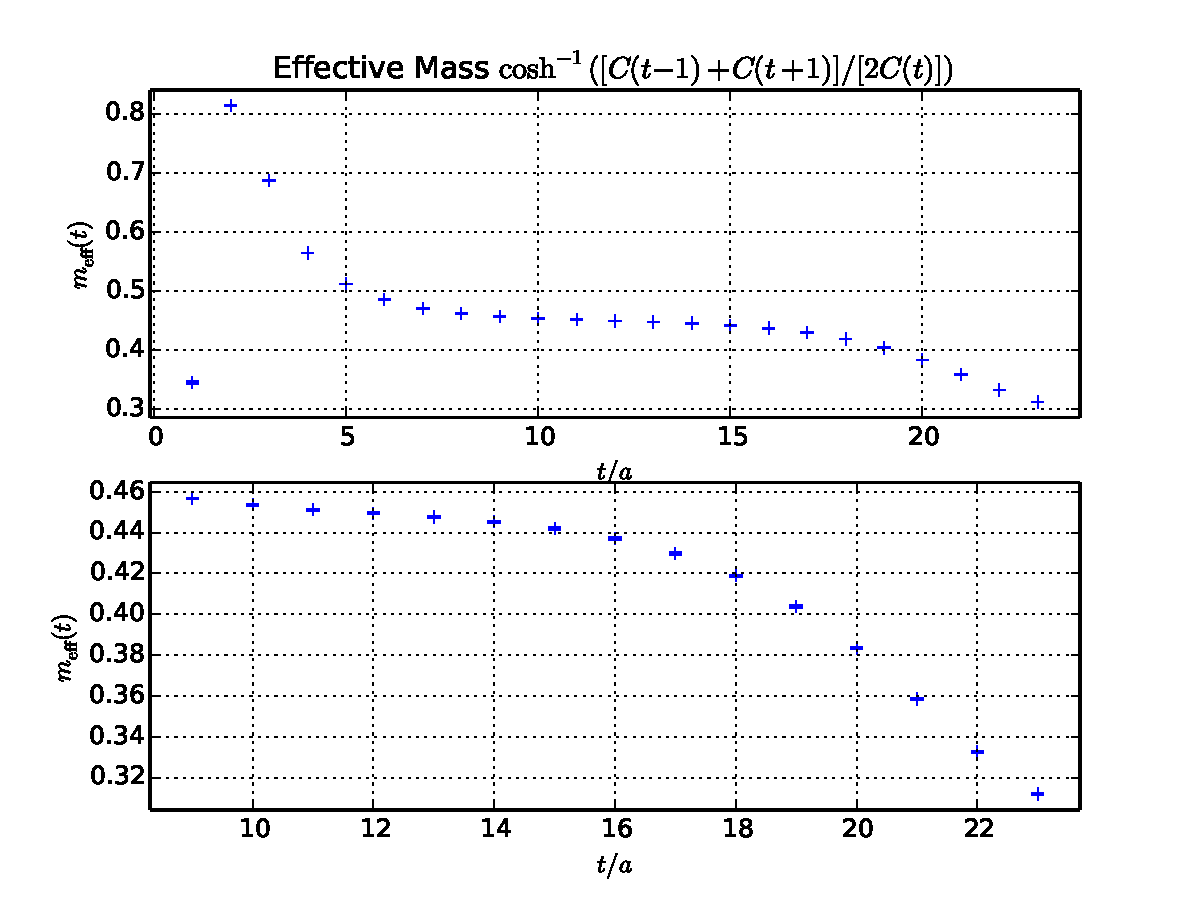
\includegraphics[height=\textheight]{plots/A100_24_L24_T48_beta190_mul0100_musig150_mudel190_kappa1632550__ev120__TB2_SO_LI6_new_c4_m_eff.pdf}
    \end{center}
\end{frame}

\subsection*{Bootstrap distribution}

\begin{frame}
    \begin{center}
        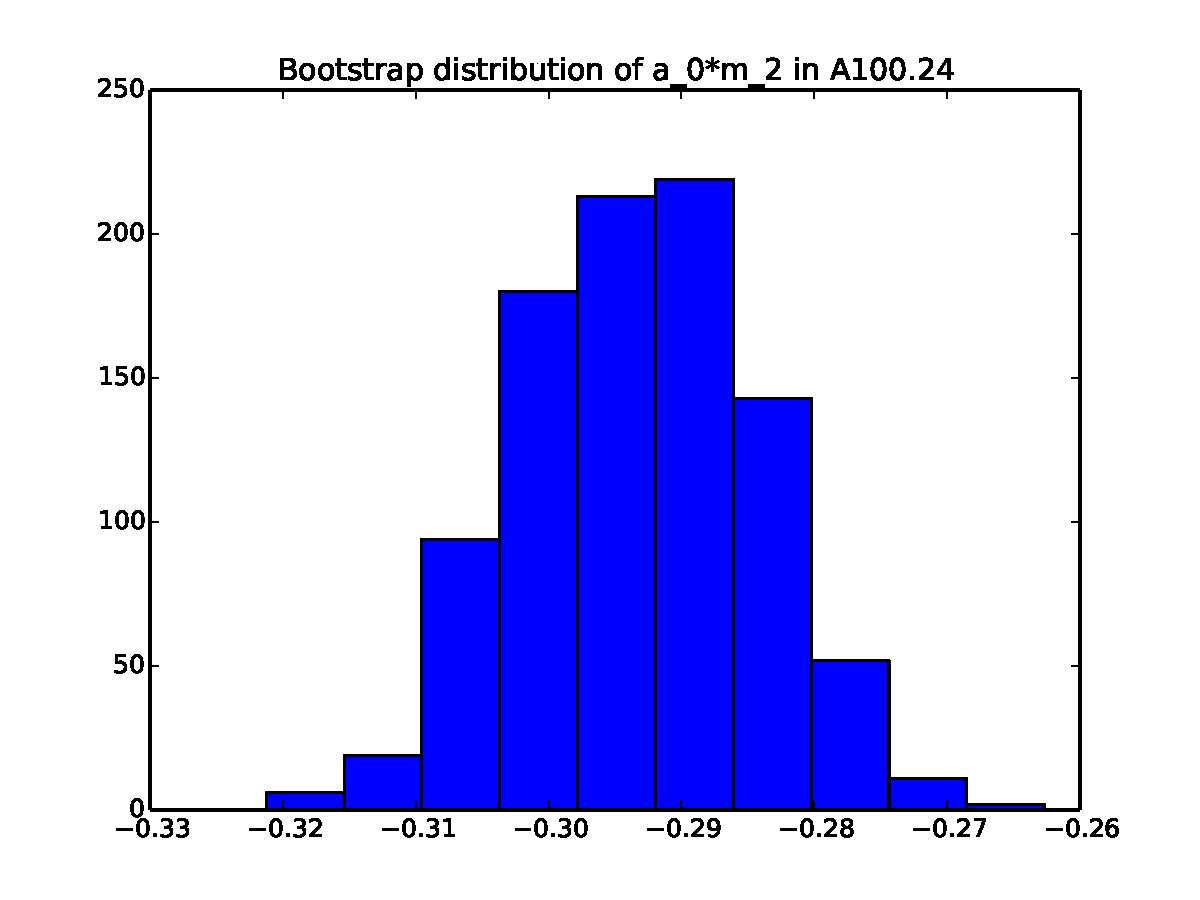
\includegraphics[height=\textheight]{plots/A100_24_L24_T48_beta190_mul0100_musig150_mudel190_kappa1632550__ev120__TB2_SO_LI6_new_boot-hist_a_0*m_2.pdf}
    \end{center}
\end{frame}

\subsection*{Extrapolation}

\begin{frame}
    \begin{center}
        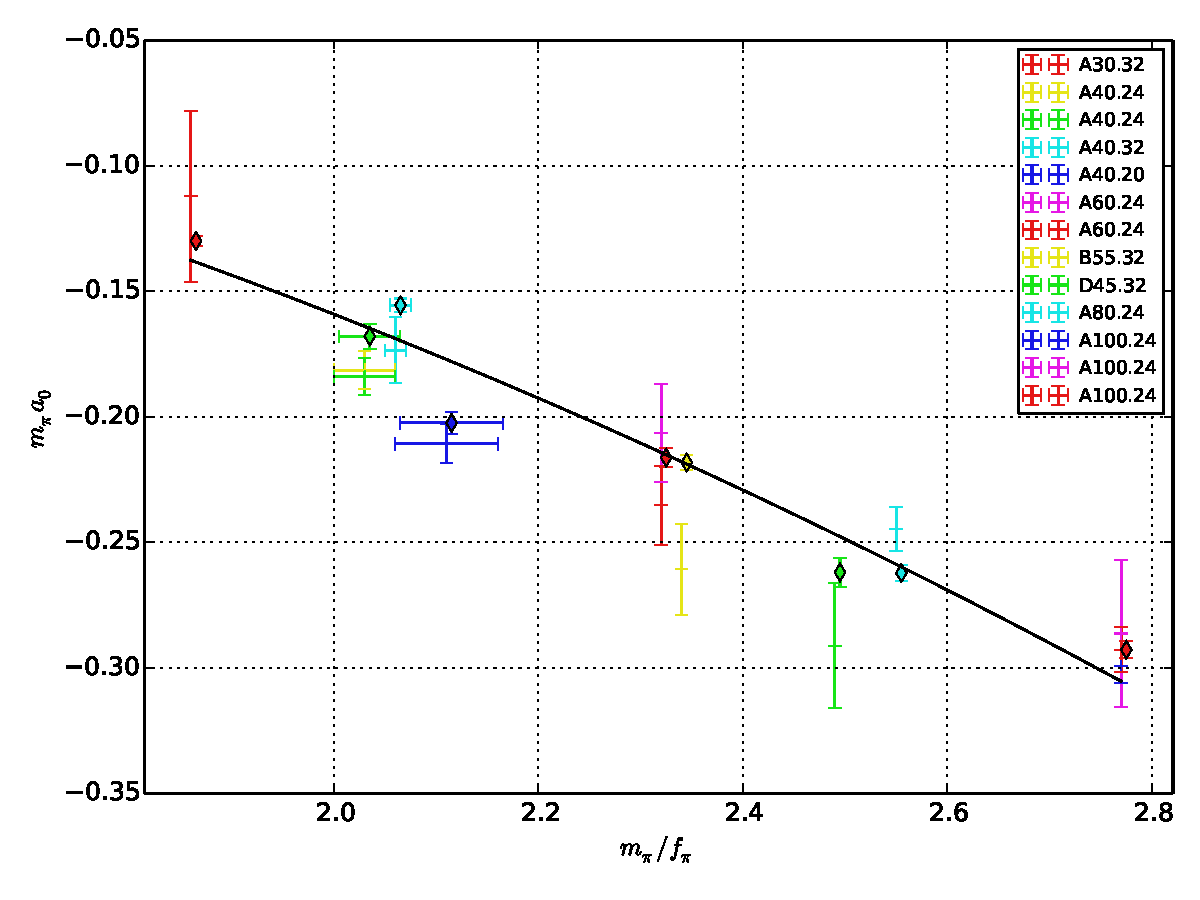
\includegraphics[height=.9\textheight]{plots/result.pdf}
    \end{center}

    Diamond data points from \parencite{Knippschild/Pi_Pi_Scattering}
\end{frame}

%%%%%%%%%%%%%%%%%%%%%%%%%%%%%%%%%%%%%%%%%%%%%%%%%%%%%%%%%%%%%%%%%%%%%%%%%%%%%%%
%                                 End matter                                  %
%%%%%%%%%%%%%%%%%%%%%%%%%%%%%%%%%%%%%%%%%%%%%%%%%%%%%%%%%%%%%%%%%%%%%%%%%%%%%%%

\section*{References}

\begin{frame}
    \frametitle{References}

    \printbibliography
\end{frame}

\section*{Download}

\begin{frame}
    \frametitle{Get the paper}

    \begin{columns}[t]
        \begin{column}{0.5\linewidth}
            To get the paper and slides, go to:
            \begin{itemize}
                \item \href{http://martin-ueding.de/en/university/msc_physics/physics760/index.html}{martin-ueding.de}
                \item University
                \item Master of Science in Physics
                \item physics760 Computational~Physics
            \end{itemize}

            \vspace{2cm}
            Made with \LaTeX\ Beamer, SciPy, matplotlib and Inkscape.
        \end{column}
        \begin{column}{0.5\linewidth}
            Or scan the code:
            \begin{center}
                
\includegraphics[width=\linewidth]{physics760.png}
            \end{center}
        \end{column}
    \end{columns}

\end{frame}

\end{document}

% vim: spell spelllang=en
